\documentclass[border=4pt]{standalone}
\usepackage{amsmath,amssymb,tikz}\usetikzlibrary{arrows.meta,fit,backgrounds}
\definecolor{figB}{RGB}{31,90,166}\definecolor{figR}{RGB}{176,48,48}\definecolor{figG}{RGB}{46,125,50}\definecolor{figO}{RGB}{214,120,20}
% T(z1,...,z6) = (0,z1,z2,0,z4,0); v1 = e1, v2 = e4, v3 = e6.
\begin{document}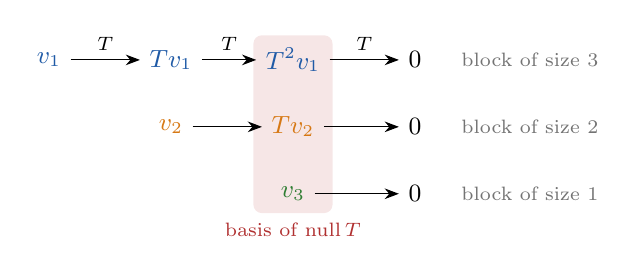
\begin{tikzpicture}[>={Stealth[length=1.8mm]},x=1.55cm,y=0.85cm,every node/.style={font=\small}]
\node[figB] (a) at (0,2) {$v_1$}; \node[figB] (b) at (1,2) {$Tv_1$}; \node[figB] (c) at (2,2) {$T^2v_1$}; \node (z1) at (3,2) {$0$};
\draw[->] (a)--(b) node[midway,above,font=\scriptsize]{$T$}; \draw[->] (b)--(c) node[midway,above,font=\scriptsize]{$T$}; \draw[->] (c)--(z1) node[midway,above,font=\scriptsize]{$T$};
\node[figO] (d) at (1,1) {$v_2$}; \node[figO] (e) at (2,1) {$Tv_2$}; \node (z2) at (3,1) {$0$};
\draw[->] (d)--(e); \draw[->] (e)--(z2);
\node[figG] (f) at (2,0) {$v_3$}; \node (z3) at (3,0) {$0$}; \draw[->] (f)--(z3);
\begin{scope}[on background layer]\node[fill=figR!12,rounded corners=3pt,inner sep=1pt,fit=(c)(e)(f)] (nt) {};\end{scope}
\node[figR,font=\scriptsize,anchor=north] at (nt.south) {basis of $\operatorname{null}T$};
\node[font=\scriptsize,black!55,anchor=west] at (3.3,2) {block of size $3$};
\node[font=\scriptsize,black!55,anchor=west] at (3.3,1) {block of size $2$};
\node[font=\scriptsize,black!55,anchor=west] at (3.3,0) {block of size $1$};
\end{tikzpicture}\end{document}
